% Section content template for individual Educative lessons
% This file contains the actual content for a specific section
% Generated from Educative API section content

% Section: Getting Ready: Library Management System
% Section ID: 5798165848784896
% Section Slug: getting-ready-library-management-system
% Generated: 2025-12-11T15:12:10.413577

A~\textbf{library management system}~\textbf{(LMS)}~aims to automate all library activities. It is software that helps manage all the primary functions of library management. With the help of a library management system, we can organize, handle, and maintain the records of numerous books and members comprehensively and systematically.
\\
A \textbf{librarian} can use this software to track the number of books in the library and retain several records, including new books, borrowed books with due dates, members who borrowed books, returned books, fines for late returned books, etc. In short, the library management system stores and updates the complete library database.
\\
LMS also supports maintaining the physical library. The user can keep track of a book's position in the library and search for whether or not the book is currently available. Therefore, LMS helps organize and retrieve library data efficiently.
\\
In this LLD interview case study, you'll focus on:

\begin{itemize}
\item
\protect\phantomsection\label{3rIwNZR0yJhHLtDjBGnVe}
Efficiently searching and managing books and other resources by various attributes (title, author, category, etc.).
\item
\protect\phantomsection\label{76bX_ZRBKUVtwu64Bpd84}
Handling book borrowing, returning, and reservation workflows.
\item
\protect\phantomsection\label{eo0GltmAG_6hGJ6XPJWxF}
Managing user roles (librarian, member) and their permissions.
\item
\protect\phantomsection\label{BAY2-PQyukd23kGWWZ7BM}
Supporting fine calculation and renewal processes for overdue and renewed books.
\end{itemize}
\\
\textbf{Note:} This system model can be adapted for academic, public, or private libraries and can support various library policies (such as special collections, inter-library loans, or different user types).

\begin{figure}[htbp]
 \centering
 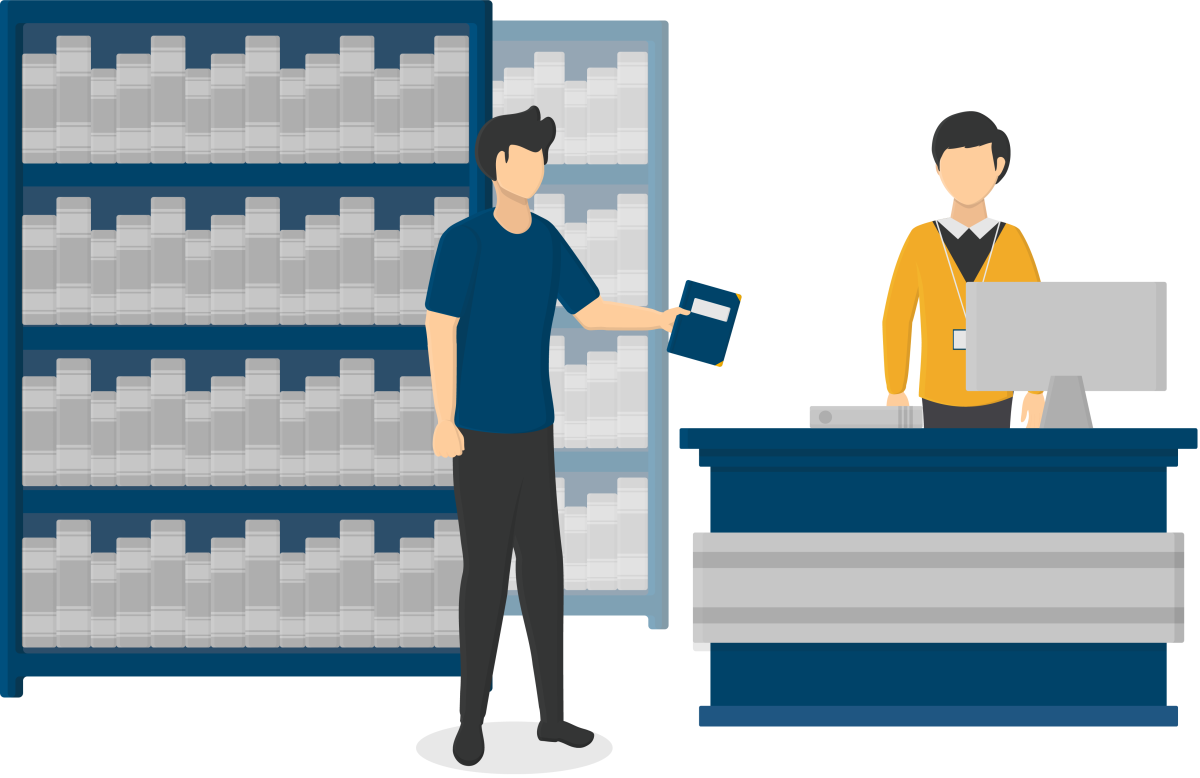
\includegraphics[width=0.25\textwidth]{Images/chapter_9/section_5798165848784896/5071505916690432.png}
 \caption{An example of the library management system}
\end{figure}

\section{Expectations from the interviewee}\label{expectations-from-the-interviewee}
\\
The LMS has multiple components, each with its specific requirements and constraints. Let 's look at some of the main expectations the interviewer will want to hear you discuss in more detail.

\subsection{Efficient searching}\label{efficient-searching}
\\
Searching for books is one of the most crucial functions of LMS. The user must be able to search for any book. Different users may want to search for a book through different methods. Therefore, the interviewer can ask questions like these:

\begin{itemize}
\tightlist
\item
Can the user search for a book using attributes other than the book name?
\item
How can the user search for a book by its author name, publication date, etc.?
\item
How will the user search a specific category of books, like magazines, journals, newspapers, etc.?
\end{itemize}

\subsection{Versatility}\label{versatility}
\\
Before designing the system, it is mandatory to specify the actors of the system. Hence , the interviewer can ask about the actors of the system as follows:

\begin{itemize}
\tightlist
\item
Can only a librarian or all library members use the software?
\end{itemize}

\subsection{Book reservation}\label{book-reservation}
\\
Another significant feature of LMS is the reservation of the book.

\begin{itemize}
\tightlist
\item
What is the mechanism of book reservation?
\item
Can a member reserve a book again if it is already reserved?
\item
How does the status of the book change when a member returns a book?
\end{itemize}

\subsection{Book renewal}\label{book-renewal}
\\
Similar to the book reservation, the interviewer can ask about the book renewal functionality with a question like this:

\begin{itemize}
\tightlist
\item
What is the mechanism of book renewal if a member wants to hold a book for longer?
\end{itemize}

\subsection{Fine management}\label{fine-management}
\\
There is another question that the interviewer may be interested in asking:

\begin{itemize}
\tightlist
\item
How is the calculation and deduction of the fine handled if the book is returned late?
\end{itemize}

\section{Design approach}\label{design-approach}
\\
We will design this library management system using the bottom-up design approach. For this purpose, we will follow the steps below:

\begin{itemize}
\item
First, we'll identify simple core entities such as Book, Member, and Librarian, and define their responsibilities.
\item
Next, we'll model book search, borrowing, return, reservation, renewal, and fine calculation workflows.
\item
We'll ensure the system supports role-based access control (RBAC) and maintains accurate transaction and catalog records.
\end{itemize}
\\
This design approach will address concurrency and scalability and follow SOLID principles to ensure maintainability and extensibility. Later , diagrams and code will illustrate major workflows and class structures.

\subsection{Design pattern~}\label{62LNh9ika4Xt1fqohoXRs}
\\
During an interview, discussing the design pattern a library management system falls under is always a good practice. Stating the design pattern gives the interviewer a positive impression and shows that the interviewee is well-versed in the advanced concepts of object-oriented design.
\\
Try to answer the following question. If you are not familiar with design patterns, don't worry! You can learn about them by asking questions like, ``Define design patterns.''

\textbf{Question:}

Which design pattern(s) should be used to design a library management system? Please elaborate on your choice(s).

Let's explore the requirements of the library management system in the next lesson.

% End of section content